\documentclass[aps, prx, nofootinbib, preprintnumbers, superscriptaddress]{revtex4-2}
\input{Setting/setting}


\begin{document}


% \title{Research notes on {\NBCPatom}}
\title{Symmetry of the NBCP}
\author{Sung-Min, Park}
\begin{abstract}
    We theoretically analyze the numerical calculation results on {\NBCPatom} 
    ({\NBCP}). 
    The effective spin Hamiltonian and their stability using classical analysis are also introduced based on the linear spin-wave theory.
\end{abstract}
\date{October 28, 2024 --- \today}


\maketitle

% \tableofcontents
 


% % \newpage
% % \begin{figure}[!b]
% %     \centering
% %     \includegraphics[width=0.9\linewidth]{Figures/VUMPS_results.pdf}
% %     \caption{Numerical calculation using VUMPS
% %     (a) $\Gamma$-perturbation 
% %     (b) PD-perturbation}
% %     \label{fig: VUMPS for NBCP}
% % \end{figure}

% % \begin{figure}[!b]
% %     \centering
% %     \begin{minipage}[t]{0.48\textwidth}
% %         \centering
% %         \includegraphics[width=\textwidth]{Figures/PD_JGamma.png}
% %         \textbf{(a)} $J_{\Gamma}$-perturbation
% %     \end{minipage}
% %     \hfill
% %     \begin{minipage}[t]{0.48\textwidth}
% %         \centering
% %         \includegraphics[width=\textwidth]{Figures/PD_JPD.png}
% %         \textbf{(b)} $J_{\rm PD}$-perturbation
% %     \end{minipage}
% %     \caption{Classical calculation for NBCP model Hamiltonian}
% %     \label{fig: classical phase diagram for NBCP}
% % \end{figure}

% % \begin{table}[!b]
% %     \centering
% %     \begin{tabular}{c|c|c|c|c|c}
% %         \hline\hline
% %         \multirow{2}{*}{Phases} &  \multicolumn{3}{c|}{Perturbation}  & \multirow{2}{*}{\# of sublattices} & \multirow{2}{*}{Ref.}\\
% %                                 & XXZ & $\Gamma$ & PD &  & \\
% %         \hline
% %         Y                       & O & O & O & \multirow{5}{*}{3} & \ref{sec: Y-phase} \\
% %         UUD                     & O & O & O &                    & \ref{sec: UUD-phase} \\
% %         $\Gamma$ (?)            & O & O & O &                    & \ref{sec: Gamma-phase} \\
% %         V                       & O & O & O &                    & \ref{sec: V-phase} \\
% %         Fully Polarized (FM)    & O & O & O &                    & \ref{sec: Fully Polarized-phase} \\
% %         \hline
% %         Helical                 & X & O & X & \multirow{3}{*}{2} & \ref{sec: Stripe-Helical-phase} \\
% %         Stripe-1 (Stripe-Y(X))  & X & X & O &                    & \ref{sec: Stripe-Y/X-phase} \\
% %         Stripe-2 (Stripe-YZ)    & X & X & O &                    & \ref{sec: Stripe-YZ-phase} \\
% %         \hline
% %         Skyrmion (\emph{new})   & X & O & X & 4 & \ref{sec: Skyrmion-phase} \\
% %         \hline
% %         Paramagnet              & X & X & O & - & \ref{sec: Paramagnet-phase} \\
% %         \hline\hline
% %     \end{tabular}
% %     \caption{Phase diagram for TLAF model with fixed XXZ model parameter: $(J_{xy}, J_{z}) = (0.076 \, \mathrm{meV}, 0.125 \, \mathrm{meV})$ with strong $z$-anisotropy $\Delta = J_{z}/J_{xy} = 1.644$. 
% %     The Ref.~\cite{PhysRevX.9.021017} studied for $0 \le \Delta = J_{z}/J_{xy} \le 1$, and find that there are other phases: 120{\textdegree} N\'eel and Dual 120{\textdegree} N\'eel.
% %     }
% %     \label{tab: Phases for NBCP}
% % \end{table}


% \newpage

% \section{PREVIEW: {\NBCP}}

% The effective spin Hamiltonian for {\NBCP} reads
% \begin{equation}\label{Eq: TLAF of NBCP}
%     \hat{H} = \hat{H}_{\NBCP} - h\sum_{j} \hat{S}_{j}^{z},
% \end{equation}
% where $h =  g_{z} \mu_{B} B \ge 0$ and $\hat{H}_{\NBCP} = \sum_{\langle i, j \rangle} h_{ij}$ is defined as follows:
% \begin{equation}\label{eq: Jab - exchange matrices}
%     h_{ij} (J_{xy}, J_{z}, J_{\rm PD}, J_{\Gamma}) 
%     = \sum_{\alpha,\beta = x,y,z} J_{\alpha \beta}^{\varphi_{ij}} \hat{S}_i^{\alpha} \hat{S}_j^{\beta}, 
%     \quad \text{ with } \quad
%     J_{\alpha\beta}^{\phi} = 
%     \begin{pmatrix}
%         J_{xy}+ 2J_{\rm PD} \cos \varphi_{ij} &   - 2 J_{\rm PD} \sin \varphi_{ij}              &   -J_{\Gamma} \sin \varphi_{ij} \\
%         -2J_{\rm PD} \sin \varphi_{ij}        &       J_{xy} - 2J_{\rm PD} \cos \varphi_{ij}    & J_{\Gamma} \cos \varphi_{ij} \\
%         -J_{\Gamma}  \sin \varphi_{ij}        &       J_{\Gamma} \cos \varphi_{ij}              & J_z
%     \end{pmatrix}, 
% \end{equation}
% Here, the indices $\alpha, \beta$ label the spin $x,y,z$ components and $J_{\rm PD} (= J_{\pm \pm})$ and $J_{\Gamma} (= J_{z \pm} )\ge 0$.
% The $\lbrace \phi \rbrace$ are link-angles, which have ${\phi : 0, 2 \pi/3, 4 \pi /3}$.
% \begin{itemize}
%     \item As Ref.~\cite{PhysRevB.94.035107} pointed out, one needs to consider only positive $J_{\Gamma} (= J_{z+} )\ge 0$.
%     This is because the global $\pi$-rotation around the $z$-axis that should leave the Hamiltonian is equivalent to changing $J_{\Gamma} \rightarrow - J_{\Gamma}$.
% \end{itemize}
% The parameters and symbols used in this note are summarized below [Table.~\ref{tab: Summary of notations}].
% \begin{table}[!h]
%     \centering
%     \begin{tabular}{c|c|c}
%         \hline\hline
%          Symbol   & Descriptions &  Reference  \\
%          \hline
%          $J_{xy}$       & $xy$                  & $0.067 \, \mathrm{meV} $ \\
%          $J_{z}$        & Ising                 & $0.125 \, \mathrm{meV} $ \\
%          $J_{\Gamma}$   & Off-diagonal symmetry & \multirow{2}{*}{(less than 0.004 meV)} \\
%          $J_{\rm PD}$   & Pseudo-Dipolar        &  \\
%          \hline
%          $g_{z}$        & Lande $g$-factor      & 4.645 \\
%          $\mu_{B}$      & Bohr magneton         & $5.788 \times 10^{-2} \, \mathrm{meV/T}$ \\
%          \hline\hline
%     \end{tabular}
%     \caption{Summary of notations}
%     \label{tab: Summary of notations}
% \end{table}


\section{Triangular Lattice Spin System}


In systems with strong spin-orbit coupling, the magnetic degrees of freedom become entangled with the orbital orientations, which are themselves locked to the crystal lattice by crystal field effects~\cite{witczak2014correlated}. 
This couplings give rise to bond-dependent interactions that respect the discrete symmetries of the lattice, thereby breaking the continuous spin-rotational symmetry in general~\cite{PhysRevB.94.035107}. 

A general form of the spin-orbit-induced anisotropic exchange Hamiltonian, relevant to a wide class of systems, is given by
\begin{equation}\label{eq: general spin exchange Hamiltonian}
    \hat{H} 
    =   % \sum_{i} \hat{\mathbf{S}}_{i}^{T} \mathbf{I}_{i} \hat{\mathbf{S}}_{i} +
    \sum_{\langle i,j \rangle} \hat{\mathbf{S}}_{i}^{T} \mathbf{J}_{ij} \hat{\mathbf{S}}_{j} 
    + \sum_{\langle\langle i, j \rangle \rangle} \hat{\mathbf{S}}_{i}^{T} \mathbf{K}_{ij} \hat{\mathbf{S}}_{j}, 
\end{equation}
where $\hat{\mathbf{S}}_i^T = (S_i^x, S_i^y, S_i^z)$ is the spin vector at site $i$, and $\langle i,j \rangle$ and $\langle\langle i, j \rangle \rangle$ denote nearest-neighbor and next-nearest-neighbor pairs, respectively. The $3 \times 3$ exchange matrices $\mathbf{J}_{ij}$ and $\mathbf{K}_{ij}$ depend on the orientation of the bond connecting sites $i$ and $j$, and the matrix elements of $\mathbf{J}_{ij}$ and $\mathbf{K}_{ij}$ are fully constrained by the space group symmetries of the underlying lattice.


\subsection{Effective Hamiltonian constrained triangular lattice symmetry}

\begin{figure}[!b]
    \centering
    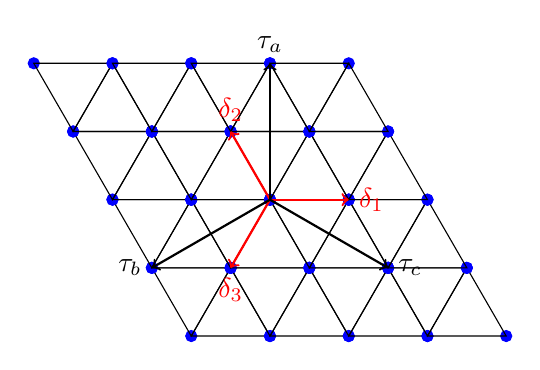
\begin{tikzpicture}
        \def\size{1}

        % 삼각형 격자 그리기: -\cols부터 \cols까지
        \foreach \x in {-2,...,1} {
            \foreach \y in {-2,...,1} {
                \pgfmathsetmacro\xa{\x * \size - \y * 0.5 * \size}
                \pgfmathsetmacro\ya{\y * \size * 0.866}

                % 삼각형의 각 꼭짓점에 파란 점 찍기
                \filldraw[blue] (\xa, \ya) circle (2pt);
                \filldraw[blue] (\xa + \size, \ya) circle (2pt); % 오른쪽 꼭짓점
                \filldraw[blue] (\xa + 0.5 * \size, \ya + 0.866 * \size) circle (2pt); % 위쪽 꼭짓점
                \filldraw[blue] (\xa - 0.5 * \size, \ya + 0.866 * \size) circle (2pt); % 위쪽 꼭짓점

                \draw (\xa, \ya) -- ++(\size, 0) -- ++(-0.5 * \size, 0.866 * \size) -- cycle;
                \draw (\xa, \ya) -- ++(-0.5 * \size, 0.866 * \size) -- ++(\size, 0) -- cycle;
            }
        }

        % delta 화살표 (중앙이 원점)
        \draw[->, thick, red] (0, 0) -- (  1 ,    0  ) node[right] {$\boldsymbol\delta_1$};    
        \draw[->, thick, red] (0, 0) -- (-0.5,  0.866) node[above] {$\boldsymbol\delta_2$};  
        \draw[->, thick, red] (0, 0) -- (-0.5, -0.866) node[below] {$\boldsymbol\delta_3$};    % 240도

        % delta 화살표 (중앙이 원점)
        \draw[->, thick, black] (0, 0) -- (  0 ,   1.732) node[above] {$\boldsymbol\tau_a$};           % 오른쪽
        \draw[->, thick, black] (0, 0) -- (-1.5, - 0.866) node[left]  {$\boldsymbol\tau_b$};     % 120도
        \draw[->, thick, black] (0, 0) -- (+1.5, - 0.866) node[right] {$\boldsymbol\tau_c$};    % 240도
        
    \end{tikzpicture}
    \caption{Triangular lattice with magnetic ions; $\boldsymbol\delta_{1,2,3}$ and $\boldsymbol\tau_{a,b,c}$ denote nearest- and next-nearest-neighbor vectors, with $\boldsymbol\delta_{1} \parallel x$ and $\boldsymbol\tau_{a} \parallel y$.}
    \label{fig: Triangular lattice spin system}
\end{figure}


Consider the Hamiltonian in Eq.~\eqref{eq: general spin exchange Hamiltonian} restricted to the nearest-neighbor $\boldsymbol{\delta}_{1}$ bond (see Fig.~\ref{fig: Triangular lattice spin system}), with the $x$-axis aligned along the bond direction:
\begin{equation}
    \hat{\mathcal{H}}_{ij} 
    \equiv \hat{\mathbf{S}}_{i}^{T} \mathbf{J}_{ij} \hat{\mathbf{S}}_{j} 
    = J_{\boldsymbol\delta_{1}}^{\alpha\beta} \hat{S}_{i}^{\alpha} \hat{S}_{j}^{\beta},
\end{equation}
where $J_{\boldsymbol\delta_{1}}^{\alpha\beta}$ is a constant matrix, and repeated indices $\alpha, \beta = x, y, z$ are summed over. Here, the $x$ and $y$ directions lie in the plane, while $z$ denotes the out-of-plane direction.
As illustrated in Fig.~\ref{fig: Triangular lattice spin system}, the lattice possesses the following symmetries: (i) site-centered inversion symmetry $\mathcal{I}$ and lattice translations $\mathcal{T}_{1,2}$ along $\boldsymbol{\delta}_{1,2}$; (ii) a twofold rotation $C_{2}$ around each bond axis; and (iii) a threefold rotation $C_{3}$ about the $z$-axis. These symmetries constrain the form of the exchange matrix by eliminating most of its elements.


\begin{enumerate}[label=(\roman*)]
    \item The inversion $\mathcal{I}_{\boldsymbol\delta_{1}}$ with respect to the center of the $\boldsymbol\delta_{1}$ bond, which is equivalent to a combination of site-centered inversion and the translation $\mathcal{T}_{1}$, preserves the form of the exchange Hamiltonian $\hat{\mathcal{H}}_{ij}$.
    \begin{equation}
        \mathcal{I}_{\boldsymbol\delta_{1}} \big[ \hat{\mathcal{H}}_{ij} \big] 
        = \mathcal{I}_{\boldsymbol\delta_{1}} \big[ J_{\boldsymbol\delta_{1}}^{\alpha\beta} \hat{S}_{i}^{\alpha} \hat{S}_{j}^{\beta} \big]
        = J_{\boldsymbol\delta_{1}}^{\alpha\beta} \hat{S}^{-\alpha}_{j} \hat{S}^{-\beta}_{i}
        = (-1)^{2} J_{\boldsymbol\delta_{1}}^{\alpha\beta} \hat{S}^{\alpha}_{j} \hat{S}^{\beta}_{i}
        = J_{\boldsymbol\delta_{1}}^{\alpha\beta} \hat{S}^{\beta}_{i} \hat{S}^{\alpha}_{j}
        = J_{\boldsymbol\delta_{1}}^{\beta\alpha} \hat{S}^{\alpha}_{i} \hat{S}^{\beta}_{j}
        \overset{!}{=} J_{\boldsymbol\delta_{1}}^{\alpha\beta} \hat{S}^{\alpha}_{i} \hat{S}^{\beta}_{j}
    \end{equation}
    Evidently, this symmetry operation corresponds to exchanging the lattice indices $i \leftrightarrow j$.


    \item The two-fold (180\textdegree) rotation about the $\boldsymbol\delta_1$ bond, denoted as $\mathcal{R}_{\boldsymbol\delta_{1}}$, inverts the $y$ and $z$ components (i.e., $y \to -y$ and $z \to -z$), while leaving the form of the exchange Hamiltonian $\hat{\mathcal{H}}_{ij}$ invariant. This requirement imposes the constraint that the off-diagonal exchange components mixing $x$ with $y$ or $z$ must vanish, namely $J_{xy} = J_{xz} = J_{yx} = J_{zx} = 0$.
    Accordingly, the exchange matrix $\mathbf{J}_{\boldsymbol\delta_{1}}$ is constrained to the form
    \begin{equation}
        \mathbf{J}_{\boldsymbol\delta_{1}} =
        \begin{pmatrix}
            J_{xx} &   0    &   0    \\
              0    & J_{yy} & J_{yz} \\
              0    & J_{zy} & J_{zz} \\
        \end{pmatrix}.
    \end{equation}
    This matrix can be conveniently reparametrized as
    \begin{equation}
        \mathbf{J}_{\boldsymbol\delta_{1}} =
        \begin{pmatrix}
            J + 2 J_{\rm PD} &   0              &   0           \\
              0              & J - 2 J_{\rm PD} & J_{\Gamma}    \\
              0              & J_{\Gamma}       & \Delta J      \\
        \end{pmatrix},
    \end{equation}
    where the parameters are defined as $J = (J_{xx} + J_{yy})/2$, $\Delta = J_{zz}/J$, $J_{\Gamma} = J_{yz}$, and $J_{\rm PD} = (J_{xx} - J_{yy})/4$.

    
    \item Invariance under $C_3$ rotation about the $z$ axis implies that the exchange matrix transforms covariantly under the rotation of the bond direction. Specifically, the exchange matrix for a bond along $\boldsymbol\delta_{a}$ is related to that of $\boldsymbol\delta_{1}$ by $\mathbf{J}_{\boldsymbol\delta_{a}} = \mathbf{R}_{a}^{-1} \mathbf{J}_{\boldsymbol\delta_{1}} \mathbf{R}_{a}$, where the rotation matrix $\mathbf{R}_{\varphi}$ is given by
    \begin{equation}
        \mathbf{R}_{\varphi} = 
        \begin{pmatrix}
              \cos \tilde{\varphi} &  \sin \tilde{\varphi} &    0   \\
            - \sin \tilde{\varphi} &  \cos \tilde{\varphi} &    0   \\
                        0          &            0          &    1
        \end{pmatrix}.
    \end{equation}
    Here, $\tilde{\varphi}$ denotes the in-plane rotation angle that maps $\boldsymbol\delta_{1}$ to $\boldsymbol\delta$. 
\end{enumerate}
As a result, the general form of the exchange matrix along an arbitrary bond direction $\boldsymbol\delta$ becomes
\begin{equation}
    \mathbf{J}_{\boldsymbol\delta} =
    \begin{pmatrix}
        J + 2 J_{\rm PD} \cos 2\tilde{\varphi} &     2 J_{\rm PD} \sin 2\tilde{\varphi} & - J_{\Gamma} \sin \tilde{\varphi} \\
            2 J_{\rm PD} \sin 2\tilde{\varphi} & J - 2 J_{\rm PD} \cos 2\tilde{\varphi} &   J_{\Gamma} \cos \tilde{\varphi} \\
          -   J_{\Gamma} \sin  \tilde{\varphi} &       J_{\Gamma} \cos  \tilde{\varphi} &   \Delta J
    \end{pmatrix}
    =
    \begin{pmatrix}
        J + 2 J_{\rm PD} \cos \tilde{\varphi} & - 2 J_{\rm PD} \sin \tilde{\varphi}     & -J_{\Gamma} \sin \tilde{\varphi} \\
        - 2 J_{\rm PD} \sin \tilde{\varphi}   & J - 2 J_{\rm PD} \cos \tilde{\varphi}   &  J_{\Gamma} \cos \tilde{\varphi} \\
        - J_{\Gamma} \sin \tilde{\varphi}     & J_{\Gamma} \cos \tilde{\varphi}         &  \Delta J
    \end{pmatrix},
\end{equation}
where the angle $\tilde{\varphi}$ takes the values $0$, $2\pi/3$, and $4\pi/3$ for the three symmetry-equivalent bond directions in the triangular lattice.


Next, consider the next-nearest-neighbor spin exchange ($\hat{\mathcal{K}}_{ij}$), which takes the form
\begin{equation}
    \hat{\mathcal{K}}_{ij} 
    = \hat{\mathbf{S}}_{i}^{T} \mathbf{K}_{ij} \hat{\mathbf{S}}_{j}.
\end{equation}
Due to the symmetries of the triangular lattice, the exchange matrix $\mathbf{K}_{ij}$ must be symmetric, i.e., $K^{\alpha\beta} = K^{\beta\alpha}$. Specifically, inversion symmetry about the bond center ($\mathcal{I}_{\boldsymbol{\tau}_{a}}$) and the 2-fold rotation around the $\boldsymbol{\tau}_a$ bond constrain the off-diagonal components involving $y$, leading to $K_{y\gamma} = K_{\gamma y} = 0$ for $\gamma = y, z$. Therefore, the form of the next-nearest-neighbor spin exchange matrix $\mathbf{K}_{\boldsymbol{\tau}_{a}}$ is given by
\begin{equation}
    \mathbf{K}_{\boldsymbol{\tau}_{a}}
    =
    \begin{pmatrix}
        K_{xx} & 0 & K_{xz} \\
        0 & K_{yy} & 0 \\
        K_{zx} & 0 & K_{zz}
    \end{pmatrix}
    =
    \begin{pmatrix}
        K + 2 K_{\rm PD} & 0                & K_{\Gamma} \\
        0                & K - 2 K_{\rm PD} & 0 \\
        K_{\Gamma}       & 0                & \Delta K
    \end{pmatrix}.
\end{equation}
For other bonds, rotational invariance yields $\mathbf{K}_{\boldsymbol{\tau}_{i}} = \mathbf{R}_{\varphi}^{T} \mathbf{K}_{\boldsymbol{\tau}_{a}} \mathbf{R}_{\varphi}$
\begin{equation}
    \mathbf{K}_{\boldsymbol{\tau}} 
    =
    \begin{pmatrix}
        K + 2 K_{\rm PD} \cos 2\tilde{\phi} &     2 K_{\rm PD} \sin 2\tilde{\phi} & K_{\Gamma} \cos \tilde{\phi} \\
            2 K_{\rm PD} \sin 2\tilde{\phi} & K - 2 K_{\rm PD} \cos 2\tilde{\phi} & K_{\Gamma} \sin \tilde{\phi} \\
              K_{\Gamma} \cos  \tilde{\phi} &       K_{\Gamma}  \sin \tilde{\phi} & \Delta K
    \end{pmatrix}
    =
    \begin{pmatrix}
        K - 2 K_{\rm PD} \sin \tilde{\phi} &   - 2 K_{\rm PD} \cos \tilde{\phi} & K_{\Gamma} \cos \tilde{\phi} \\
          - 2 K_{\rm PD} \cos \tilde{\phi} & K + 2 K_{\rm PD} \sin \tilde{\phi} & K_{\Gamma} \sin \tilde{\phi} \\
              K_{\Gamma} \cos \tilde{\phi} &       K_{\Gamma} \sin \tilde{\phi} & \Delta K
    \end{pmatrix},
\end{equation}
where the bond angle $\tilde{\phi}$ takes $\tilde{\phi} = \pi/2, 7\pi/6, 11\pi/6$ and we use the fact $\sin 2\tilde{\phi} = - \cos \tilde{\phi}$ and $\cos 2\tilde{\phi} = - \sin \tilde{\phi}$.


\begin{enumerate}[label = (\roman*)]
    \item The inversion $(\mathcal{I}_{\boldsymbol\tau_{a}})$ with respect to the center of the bond, which is a combination of the site inversion and $\mathcal{T}_{1}$ translation, should leave the form of $\hat{\mathcal{K}}_{ij}$ invariant. This leads to the condition
    \begin{equation}
        \mathcal{I}_{\boldsymbol\tau_{a}} \big[ \hat{\mathcal{K}}_{ij} \big] 
        = K_{\boldsymbol\tau_{a}}^{\beta\alpha} \hat{S}^{\alpha}_{i} \hat{S}^{\beta}_{j}
        \overset{!}{=} K_{\boldsymbol\tau_{a}}^{\alpha\beta} \hat{S}^{\alpha}_{i} \hat{S}^{\beta}_{j},
    \end{equation}
    which implies $K^{\alpha\beta} = K^{\beta\alpha}$. This symmetry corresponds to exchanging the site indices $i \leftrightarrow j$.
    
    \item The 2-fold (180\textdegree) rotation around the $\boldsymbol\tau_{a}$ bond ($\mathcal{R}_{\boldsymbol\tau_{a}}$) changes $y \to -y$ and $z \to -z$, but the form of $\hat{\mathcal{K}}_{ij}$ should remain invariant. This leads to
    \begin{equation}
        \mathcal{R}_{\boldsymbol\tau_{a}} [ \hat{\mathcal{K}}_{ij} ]
        = - K_{\boldsymbol\tau_{a}}^{y\gamma} \hat{S}_{i}^{y} \hat{S}_{j}^{\gamma}
        \overset{!}{=} K_{\boldsymbol\tau_{a}}^{y\gamma} \hat{S}_{i}^{y} \hat{S}_{j}^{\gamma}
        \qquad \text{for } \gamma = y, z,
    \end{equation}
    which implies $K_{y\gamma} = K_{\gamma y} = 0$ for $\gamma = y, z$.
\end{enumerate}



% Mapping of 2D Triangular Lattice Quantum XXZ Model to Nonlinear Sigma Model and BKT Transition


\end{document}
